Pas vérifié

\subsection*{Formule de Burnside}

Si $g \in G$, $Fix(g) = \{ x \in E \mid g \cdot x = x \} \subset E$.

\begin{theorement}
Supposons $G, E$ finis, et soit $N$ le nombre d'orbites.
Alors \[ N = \sum_{g \in G} |Fix(g)| \times \frac{1}{|G|} \]
\end{theorement}

\textbf{Dém :} Soit $F = \{ (g,x) \in G \times E \mid g \cdot x = x \}$.

\noindent\begin{minipage}{0.65\textwidth}
\begin{align*}
|F| &= \sum_{g \in G} |\{ x \in E \mid g \cdot x = x \}| \quad \text{(Fubini)} \\
    &= \sum_{g \in G} |Fix(g)| \\
    &= \sum_{x \in E} \underbrace{|\{ g \in G \mid g \cdot x = x \}|}_{|G_x| \text{ (stabilisateur)}} \\
    &= \sum_{i=1}^N \sum_{x \in \mathcal{O}(x_i)} |G_{x_i}|
\end{align*}
Note : $|G| = |\mathcal{O}(x_i)| \times |G_{x_i}| \implies |G_{x_i}| = \frac{|G|}{|\mathcal{O}(x_i)|}$.
\begin{align*}
    &= \sum_{i=1}^N |\mathcal{O}(x_i)| \times \frac{|G|}{|\mathcal{O}(x_i)|} \\
    &= \sum_{i=1}^N |G| = N \times |G|
\end{align*}
\end{minipage}%
\begin{minipage}{0.35\textwidth}
\centering
\begin{tikzpicture}[scale=0.8]
    % Axes
    \draw[->] (0,0) -- (4,0) node[below] {$G$};
    \draw[->] (0,0) -- (0,3) node[left] {$E$};
    
    % Forme F (blob)
    \draw[thick] plot [smooth cycle] coordinates {(1.5,1) (2.5,0.8) (3.2,1.5) (2.8,2.2) (1.2,1.8)};
    \node at (2.8, 2.5) {$F$};
\end{tikzpicture}
\end{minipage}

\vspace{0.5cm}

\begin{exemple}
\textbf{Application :} Si $\sigma \in S_n$, $Fix(\sigma) = \{ i \in [\![ 1, n ]\!] \mid \sigma(i) = i \}$.

$S_n$ agit sur $[\![ 1, n ]\!]$, $i \in [\![ 1, n ]\!]$, $\sigma \cdot i = \sigma(i)$.
$\hookrightarrow$ action transitive, donc $N=1$.

Ainsi $1 = \frac{\sum_{\sigma \in S_n} |Fix(\sigma)|}{n!} \implies$ une permutation aléatoire a en moyenne un pt fixe.
\end{exemple}

\begin{exemple}
\textbf{Application 2 :} Soit $G$ un groupe fini agissant transitivement sur $E$, $|E| \geqslant 2$.

Mq $\exists g \in G$ tq $Fix(g) = \varnothing$.
\end{exemple}

\noindent \textbf{Dém :}
\[ 1 = \frac{\sum_{g \in G} |Fix(g)|}{|G|} \]
Or si $g=e$, $|Fix(e)| = |E| \geqslant 2$.

Alors absurde si $\forall g \in G, |Fix(g)| \geqslant 1$, alors $\frac{\sum_{g \in G} |Fix(g)|}{|G|} > 1$.

\vspace{0.5cm}

\begin{exemple}
    \textbf{Application 3 : Lemme de Cauchy, oral ENS 2023}
Soit $G$ un groupe fini. Soit $p \in \mathbb{P}$ tq $p \mid |G|$.\\
Alors $\exists x \in G$ d'ordre $p$.
\end{exemple}

\noindent \textbf{Démonstration :}
\[ E = \{ (x_1, \dots, x_p) \in G^p \mid x_1 x_2 \dots x_p = e \} \]
Soit $\sigma \in S_p$, $\sigma = (1, 2, 3, \dots, p)$. $H = \{ id, \sigma, \sigma^2, \dots, \sigma^{p-1} \} \hookrightarrow$ isomorphe à $\mathbb{Z}/p\mathbb{Z}$.

Soit $(x_1, \dots, x_p) \in E$.
\[ \sigma(x_1, x_2, \dots, x_p) = (x_2, x_3, \dots, x_p, x_1) \in E \]
Donc $H$ agit sur $E$.

\[ |E| = \sum_{i=1}^N |\mathcal{O}(y_i)| \quad \text{notons } n = |G| \text{ et } p \mid |G|. \]

\[ E = \{ (x_1, \dots, x_p) \in G^p \mid \underbrace{x_1 \dots x_{p-1}}_{\text{arbitraires}} \cdot \underbrace{x_p}_{\text{inverse}} = e \} \]
Donc $|E| = n^{p-1}$.

\[ |\mathcal{O}(y_i)| = |H|/|H_{y_i}| = p \text{ ou } 1. \]
(car $H$ iso à $\mathbb{Z}/p\mathbb{Z}$, $H_{y_i}$ sous-groupe de $H$ donc iso à $\mathbb{Z}/p\mathbb{Z}$. Or $p$ premier donc $\{e\}$ ou $\mathbb{Z}/p\mathbb{Z}$).

Et $|E|$ multiple de $p$, $|\mathcal{O}(y_i)| = p \text{ ou } 1$.
\[ |E| = \sum_{i=1}^N |\mathcal{O}(y_i)| = \alpha p + N_{\text{1 elt}} \]
Comme $|E|$ est multiple de $p$, alors $N_{\text{1 elt}}$ est multiple de $p$.

Soit $(x_1, \dots, x_p) \in E$.
\[ \mathcal{O}((x_1, \dots, x_p)) = \{(x_1, \dots, x_p)\} \]
\[ \sigma(x_1, \dots, x_p) = (x_1, \dots, x_p) = (x_2, x_3, \dots, x_p, x_1) \implies x_1 = x_{i+1} \]
C'est-à-dire $x_1 = x_2 = \dots = x_p$.

Comme $(e, \dots, e) \in E$ est un point fixe, $N_{\text{1 elt}} \geqslant 1$.
Comme $p \mid N_{\text{1 elt}}$, alors $N_{\text{1 elt}} \geqslant p$.
Il existe donc $x \neq e$ tel que $(x, \dots, x) \in E$, soit $x^p = e$.

\noindent donc $x = x_1 \quad \forall i, \quad x^p = e$.

Si j'ai une telle orbite, $\text{ord}(x) = p$ (si orbite de card $1 \iff x=e$).

Ce nombre non nul d'orbites de cardinal 1, car $(e, e, \dots, e)$ est invariant, est multiple de $p$.
Donc il y a au moins une autre orbite de cardinal 1, avec $x \neq e$.
\hfill \faCheckCircle

\vspace{1cm}

\section*{Coloriages}

\begin{center}
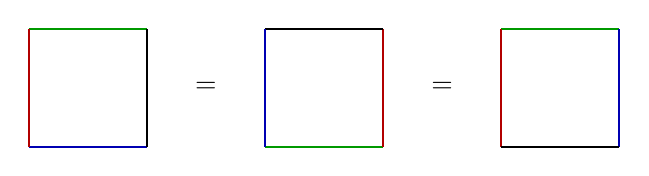
\begin{tikzpicture}[scale=1.5]
    % Carré 1
    \draw[thick, green!60!black] (0,1) -- (1,1); % Haut
    \draw[thick, blue!70!black] (0,0) -- (1,0);  % Bas
    \draw[thick, red!70!black] (0,0) -- (0,1);   % Gauche
    \draw[thick, black] (1,0) -- (1,1);           % Droite
    
    \node at (1.5, 0.5) {$=$};
    
    % Carré 2 (Rotated slightly to mimic handwriting style or just different color config?) 
    % The drawing shows a rotated square, implying symmetry check.
    \begin{scope}[shift={(2,0)}]
        \draw[thick, green!60!black] (0,0) -- (1,0);
        \draw[thick, red!70!black] (1,0) -- (1,1);
        \draw[thick, black] (0,1) -- (1,1);
        \draw[thick, blue!70!black] (0,0) -- (0,1);
    \end{scope}
    
    \node at (3.5, 0.5) {$=$};
    
    % Carré 3
    \begin{scope}[shift={(4,0)}]
        \draw[thick, green!60!black] (0,1) -- (1,1);
        \draw[thick, red!70!black] (0,0) -- (0,1);
        \draw[thick, blue!70!black] (1,0) -- (1,1);
        \draw[thick, black] (0,0) -- (1,0);
    \end{scope}
\end{tikzpicture}
\end{center}

$E = \{ \text{tous les coloriages possibles} \}$, $|E| = 3^4$ (3 couleurs, 4 côtés).

Il y a un groupe qui agit sur $E$, $G = \{ \text{symétries du carré} \}$.
\begin{align*}
    G &= \{ id, r_{\pi/2}, r_{-\pi/2}, -id, s_{\text{ax}_1}, s_{\text{ax}_2}, s_{\text{diag}_1}, s_{\text{diag}_2} \} \\
    &\text{(où } -id = r_\pi \text{ est la symétrie centrale)}
\end{align*}

$G = D_4$, groupe diédral à 8 éléments.

Nb d'orbites pour l'action de $G=D_4$ sur $E$ ? $\hookrightarrow$ nb de coloriages.

\[ N = \text{nb de coloriages différents} = \frac{\sum_{g \in G} |Fix(g)|}{|G|} \]
avec $|G|=8$.

\begin{center}
\renewcommand{\arraystretch}{1.5}
\begin{tabular}{c|l}
    $g$ & $|Fix(g)|$ \\
    \hline
    $id$ & $3^4$ \\
    \hline
    $r_{\pm \pi/2}$ & $3$ (1 seule couleur) \\
    \hline
    $s_{\text{ax } 1,2}$ & $3^3$ \\
    \hline
    $s_{\text{diag}}$ & $9$ \\
    \hline
    $-id$ & $3^2$
\end{tabular}
\end{center}

\[ \implies 21 \text{ coloriages}. \]

\section*{Cauchy dans le cas abélien}

$G$ abélien, $p \mid |G|$, on veut un élément d'ordre $p$.

\textbf{Fait :} Si $x \in G$ d'ordre $kp$, $x^k$ est d'ordre $p$.

\textbf{Absurde :} Aucun élément n'a un ordre multiple de $p$.

Soit $G = \{g_1, \dots, g_n\}$, et $m = \text{ppcm}(\text{ordre}(g_i))$.

Considérons l'application :
\begin{align*}
    (\mathbb{Z}/m\mathbb{Z})^n &\longrightarrow G \\
    (a_1, \dots, a_n) &\longmapsto g_1^{a_1} \dots g_n^{a_n}
\end{align*}
$\hookrightarrow$ morphisme de groupes surjectif.

D'après le théorème d'isomorphisme :
\[ (\mathbb{Z}/m\mathbb{Z})^n / \ker \varphi \simeq \text{Im } \varphi = G \]

Passons aux cardinaux :
\[ |(\mathbb{Z}/m\mathbb{Z})^n| = |G| \times |\ker \varphi| \]
\[ m^n = |G| \times |\ker \varphi| \]

Or $p \mid |G|$ donc $p \mid m^n \implies$ absurde.
\textit{(Car si aucun élément n'a un ordre multiple de $p$, alors $p$ ne divise pas $m$, donc $p$ ne divise pas $m^n$).}

\vspace{1cm}

\begin{exemple}
    \textbf{Exercice}
Dans le cas non abélien, faire agir $G$ sur lui-même par conjugaison.
\end{exemple}